\section{Support Vector Machine}
\textit{Manuel Dudda, Benjamin Weißer}

Die Support Vector Machine (SVM) ist eine Methode des überwachten Lernens zum Erstellen eines linearen Klassifikators. 
Ein Klassifikator bestimmt für einen gegebenes Datum eine zugehörige Zuteilung (Klasse). Mit einem Satz von Daten (Merkmalsvektoren) inklusive dessen Klassenzugehörigkeiten wird eine mathematische Trenngerade generiert, die die Daten räumlich in zwei Klassen trennt. 
Im Gegensatz zu MLPs wird die Anpassung der Trennung nicht empirisch durch Trainingsmethoden, sondern durch die Datengrundlage mathematisch optimal ermittelt. 
Dabei wird der Abstand zu den nächstliegenden Daten, den sogennanten Stützvektoren der Klassenräume, maximiert.


\begin{wrapfigure}{r}{0.48\textwidth}
	\vspace{-30pt}
	\begin{center}
		 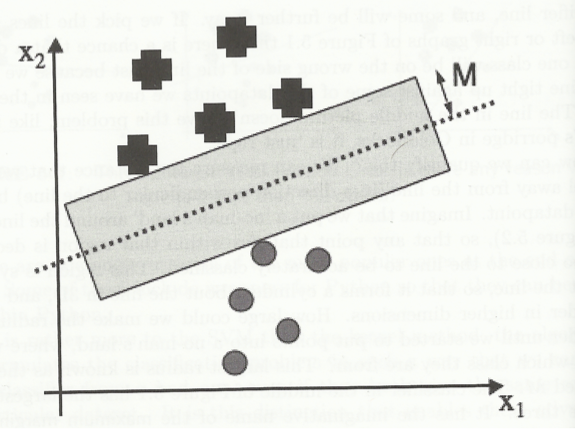
\includegraphics[width=0.48\textwidth]{svm_1.png}
	\end{center}
	\vspace{-15pt}
	\caption{linear separierte Merkmalsvektoren}
	\vspace{-15pt} 
\end{wrapfigure}

Durch dieses Optimierungskriterium ist die Trennlinie eindeutig. 
Ist die Entscheidungsgrenze gefunden, lassen sich neue Daten durch die Zuordnung eines Merkmalsvektors in den jeweiligen Klassenraum schnell klassifizieren, d. h. ob der Punkt oberhalb oder unterhalb der Trennlinie ist.

Die Support Vector Machine ist somit ein binärer Klassifikator, der die Daten lediglich in 2 Klassen unterteilen kann. 
Für eine Klassifikation von mehreren Klassen wurden Strategien entwickelt, die das Prinzip der SVM erweitern. 
Eine dieser Strategien ist die Kombination von mehreren SVMs von “Einer gegen den Rest-Klassifikatoren”. 
Als Klassifikation wird die SVM mit dem höchsten Ergebnis gewählt (“winner takes it all”).

Ein Problem entsteht, wenn die gegebenen Merkmalsdaten nicht durch eine Trennline (Hyperbene) trennbar sind, sondern die Trennung der Daten nur durch eine Kurve o. Ä. beschrieben werden kann. 
Für die Lösung nichtlinear separierbarer Probleme bedient sich die SVM des Kernel-Tricks aus der RKHS-Theorie (Reproducing Kernel Hilbert Spaces). 
\begin{wrapfigure}{l}{0.45\textwidth}
	\vspace{-30pt}
	\begin{center}
	    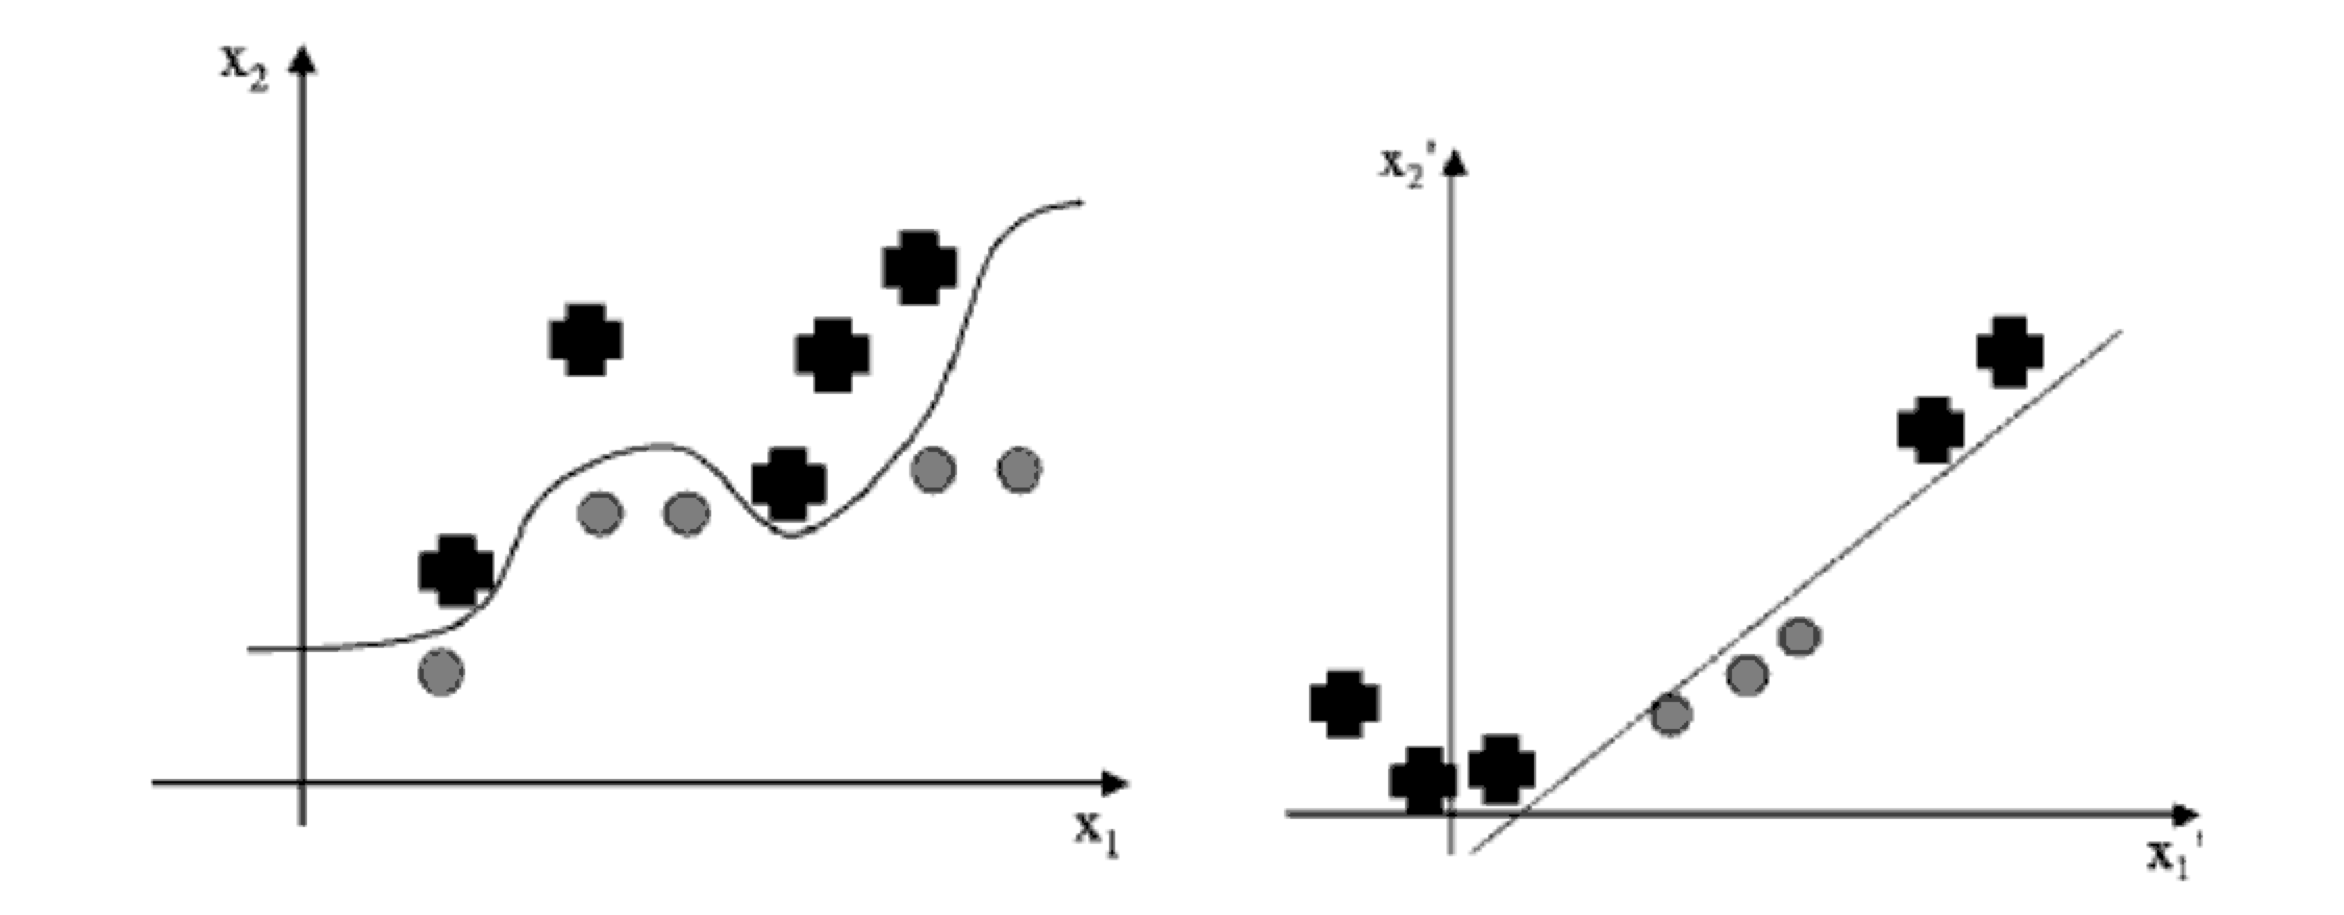
\includegraphics[width=0.45\textwidth]{svm_2.png}
	\end{center}
	\vspace{-15pt}
	\caption{transformierte Merkmalsvektoren}
		\vspace{-65pt}
\end{wrapfigure}
Eine Kernel-Funktion transformiert die Merkmalsvektoren in einen höherdimensionalen (Hilbert-)Raum, in dem die evaluierten Daten sodann linear separierbar sind.


\newpage

\subsection{Implementierung}

Das “scikit-learn”-Paket von den “scikit-learn developers” steht frei unter BSD License für Python zur Verfügung. 
Es beinhaltet viele komfortable Bibliotheken zum Thema Machine Learning. 
Für unsere Zwecke benutzen wir die vorgefertigten SVM-Algorithmen. 
Diese berücksichtigen freundlicherweise bereits die Features für die Klassifizierung mehrerer Klassen sowie den Kernel-Trick. Eine SVM wird folgendermaßen trainiert:

\begin{lstlisting}
import numpy as np#
from sklearn import svm#

X = np.array([[-1,1],[1,1],[1,-1],[-1,-1]])
y = [1,-1,1,-1]

#Train SVM
clf = svm.SVC(kernel='linear')
clf.fit(X, y)#

#Predict
print clf.predict([0.2,0.2])#
print clf.predict([-0.2,0.2])#
print clf.predict([-0.2,-0.2])#
print clf.predict([0.2,-0.2])#
\end{lstlisting}


\subsection{Vorverarbeitung der Eingabedaten}

Kernpunkt der Gestenerkennung ist die anliegende Grundfrequenz von 18 kHz. 
Die aktuelle Implementierung der Gestenerkennung setzt ein Audiosignal mit einer Länge von 320 ms voraus. 
Innerhalb dieser 320 ms werden 32 Merkmalsvektoren mit einer zeitlichen Dauer von 1 ms gespeichert in einem Intervall von je 10 ms. 
Diese zeitlich versetzten 32 Merkmalsvektoren mit je 64 Datenpunkten einer Geste werden vor der Eingabe in eine trainierte SVM zuerst normalisiert. 
Dazu gibt es zwei grundlegende Ansätze:

- alle 32 Merkmalsvektoren werden mit einem “globalen” Maximalwert über alle 32 Datensätze in den Bereich zwischen 0 und 1 normalisiert\newline

- alle 32 Merkmalsvektoren werden mit ihrem jeweiligen Maximalwert in den Bereich zwischen 0 und 1 normalisiert

Letztere Methode sorgt dafür, dass die Grundfrequenz der Gestenerkennung von 18 kHz in allen Merkmalsvektoren in einem Maximalwert von 1 resultiert. 
In einem nächsten Schritt bietet es sich an, diese Grundfrequenz, die ebenfalls nach der gleichen Methode normalisiert wurde, von den Merkmalsvektoren abzuziehen. 
Dadurch wird die reine Frequenzverschiebung der Geste gut sichtbar und man erhält eine sehr gute Eliminierung von Stördaten. 
Anschließend bietet es sich allerdings an, die Merkmalsvektoren erneut in den Bereich zwischen [0, 1] zu skalieren, da durch die Subtraktion der Grundfrequenz negative Werte entstehen können.


\subsection{Eingabe in die SVM}

Die zeitlich versetzten 32 Merkmalsvektoren mit je 64 Datenpunkten einer Geste können für die Eingabe in eine trainierte SVM linear aneinandergehängt werden, so dass ein einziger Eingabevektor mit 32*64 = 2048 Elementen entsteht. 
Dieses Vorgehen ist nicht kritisch, da wir die Zeitkomponente bei einer SVM nicht näher betrachten müssen. 
Sie wird indirekt durch die Position in unserem Eingabevektor berücksichtigt.

Im folgenden ist eine geplottete Aufnahmen einer Gesten zu erkennen. 
Die oberen vier Zeilen zu je acht Graphen sind die zeitlich aufeinanderfolgenden 32 Merkmalsvektoren. 
Der blaue Graph hierbei ist der normalisierte Merkmalsvektor, während die roten Graphen jeweils das Ergebnis von Merkmalsvektor - Grundfrequenz beinhalten. 
Die Grundfrequenz wurde aus insgesamt 12 verschiedenen Aufnahmen zu je 32 Merkmalsvektoren (insgesamt 384 Merkmalsvektoren) gemittelt. 
Sie ist als grüner Graph in den Bildern zu sehen.

\begin{figure}[h!]
  \centering
    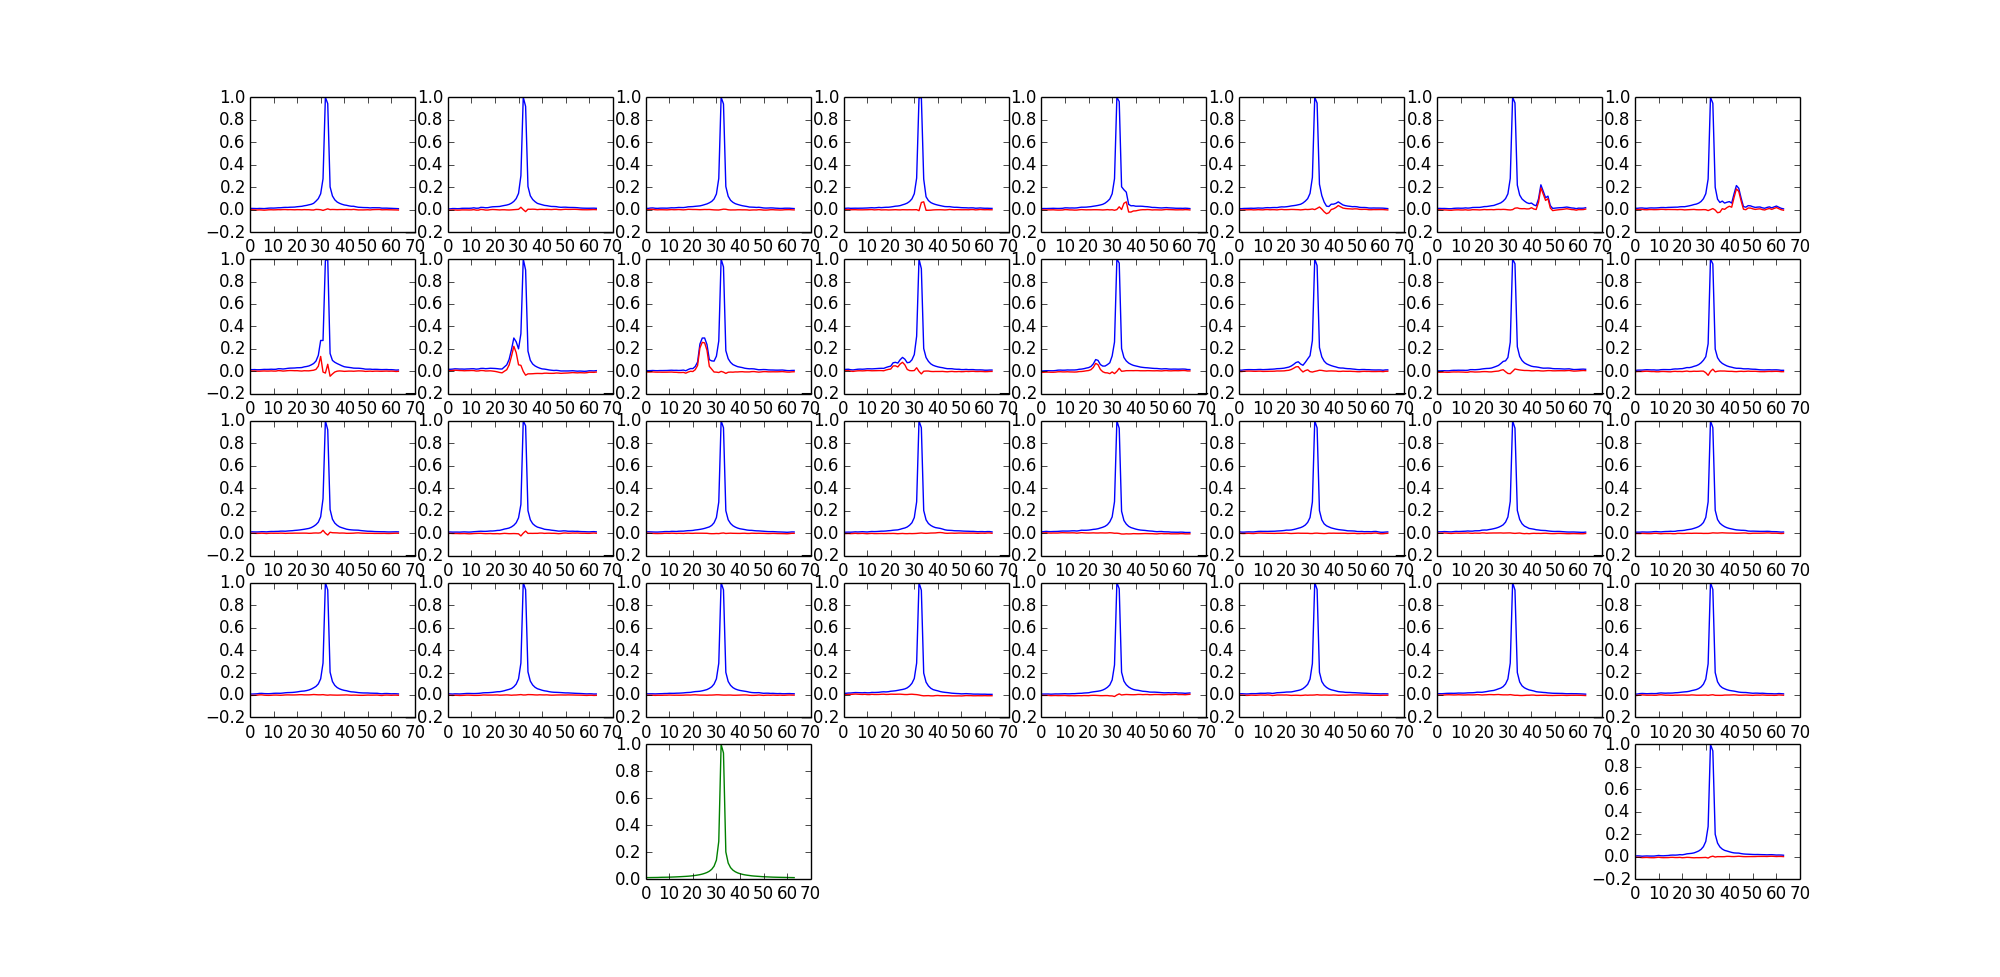
\includegraphics[width=0.8\textwidth]{svm_data_1.png}
  \caption{Ausgabe der (transformierten) Merkmalsvektoren}
\end{figure}

